\section{Introduction}
\lipsum[1] Here are some references (\cite{almero2021,borenstein1992,cazenave2014,coro2021}) and an example how to introduce an abbreviation for \ac{NAL}.

\begin{figure}
    \centering
    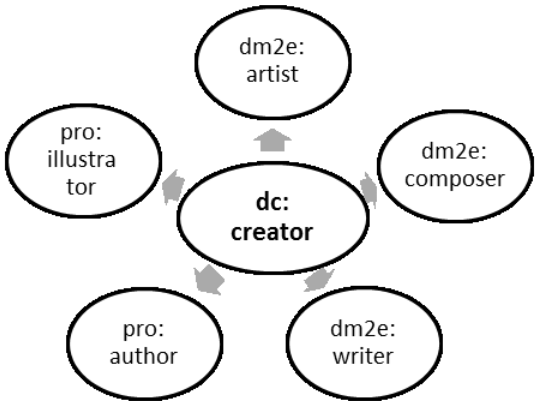
\includegraphics[width=0.6 \textwidth]{images/exampleFigure.png}
    \caption{Example Image (Origin: \href{https://isi2025.informationswissenschaft.org/wp-content/uploads/2024/05/Formatierungshinweise_ISI_2025.pdf}{ISI 2025})}
    \label{fig:exampleFigure}
\end{figure}

\subsection{First Subsection}
\lipsum[2]

\subsubsection{First SubSubsection}
\lipsum[3]

\lipsum[5]

\begin{table}[h]
	\centering
	\caption{Example Table}\label{tab:exampleTable}
		\begin{tabular}{|l|r|r|}
			\hline
			\multicolumn{1}{|c|}{\textbf{Component Name}} & \multicolumn{1}{c|}{\textbf{Acquisition Costs}} \\ \hline
			Camera Housing                                & 115.61 EUR  \\
			Mounting Frame                                & 36.65 EUR  \\
			Infrared Lighting                             & 6.68 EUR    \\
			Raspberry Pi Zero 2 W                         & 30.00 EUR   \\
			Camera Module                                 & 54.41 EUR    \\
            \hline
			\textbf{Total}                                & 349.62 EUR    \\ 
            \hline
		\end{tabular}
\end{table}
